\documentclass[letter]{article} 
\addtolength{\hoffset}{-2.25cm}
\addtolength{\textwidth}{4.5cm}
\addtolength{\voffset}{-3.25cm}
\addtolength{\textheight}{5cm}
\setlength{\parskip}{0pt}
\setlength{\parindent}{0in}

\usepackage[square,sort,comma,numbers]{natbib}
\usepackage{blindtext} % Package to generate dummy text
\usepackage{charter} % Use the Charter font
\usepackage[utf8]{inputenc} % Use UTF-8 encoding
\usepackage{microtype} % Slightly tweak font spacing for aesthetics
\usepackage{amsthm, amsmath, amssymb, setspace} % Mathematical typesetting
\usepackage{float} % Improved interface for floating objects
\usepackage{hyperref} % For hyperlinks in the PDF
\usepackage{graphicx, multicol} % Enhanced support for graphics
\usepackage{xcolor} % Driver-independent color extensions
\usepackage{pseudocode} % Environment for specifying algorithms in a natural way
\usepackage[ddmmyyyy]{datetime} % Uses YEAR-MONTH-DAY format for dates
\usepackage[spanish, activeacute, es-lcroman]{babel}

\usepackage{fancyhdr} % Headers and footers
\pagestyle{fancy} % All pages have headers and footers
\fancyhead{}\renewcommand{\headrulewidth}{0pt} % Blank out the default header
\fancyfoot[L]{} % Custom footer text
\fancyfoot[C]{} % Custom footer text
\fancyfoot[R]{\thepage} % Custom footer text
\newcommand{\note}[1]{\marginpar{\scriptsize \textcolor{red}{#1}}} % Enables comments in red on margin

\makeatletter
\renewcommand\subsection{\@startsection{subsection}{3}{\z@}%
                                     {-3.25ex\@plus -1ex \@minus -.2ex}%
                                     {-1.5ex \@plus -.2ex}% Formerly 1.5ex \@plus .2ex
                                     {\normalfont\normalsize\bfseries}}
\makeatother

\usepackage{listings}
\lstloadlanguages{[5.2]Mathematica}

\usepackage{enumerate}

\usepackage{subcaption}

\usepackage{dsfont}

\usepackage{wrapfig}

\usepackage{enumitem}

\usepackage{cancel}

\usepackage{booktabs}

%----------------------------------------------------------------------------------------


%-------------------------------
%	TITLE VARIABLES (identify your work!)
%-------------------------------

\newcommand{\firstname}{Nicolas Maldonado Baracaldo}
\newcommand{\firstid}{201423809}
\newcommand{\firstemail}{n.maldonado10@uniandes.edu.co}

\begin{document}

%-------------------------------
%	TITLE SECTION (do not modify unless you really need to)
%-------------------------------
\fancyhead[C]{}
\hrule \medskip
\begin{minipage}{0.295\textwidth} 
\raggedright
\footnotesize
\firstname \hfill\\ 
\firstid \hfill\\ 
\firstemail \hfill\\
\end{minipage}
\begin{minipage}{0.4\textwidth} 
\centering 
\large 
Introducción a los Modelos Matemáticos en Gestión Financiera (MATE2714)\\ 
\normalsize
Rene Joaquin Meziat Velez\\
Proyecto 2\\ 
\end{minipage}
\begin{minipage}{0.295\textwidth} 
\raggedleft
30 de noviembre de 2020\hfill\\
\end{minipage}
\medskip\hrule 
\bigskip

%-------------------------------
%	ASSIGNMENT CONTENT (add your responses)
%-------------------------------

\bigskip

\begin{enumerate}

\item \emph{Considere un activo cuyo precio sigue un camino aleatorio dado por: $dS = \mu Sdt + \sigma SdX$ donde $dX$ es una variable aleatoria con distribución normal de media nula y varianza $dt$ (proceso de Wiener). Utilice un entorno computacional para simular este camino aleatorio con diferentes valores de la tendencia $\mu$ y de la desviación estándar $\sigma$, a partir de un precio inicial $S_0$. Usted debe realizar un programa que le permita al usuario cambiar estos parámetros y ejecutar la simulación para obtener otros posibles resultados.}

\medskip

\textbf{\textit{Sol.}} Se escribió en \texttt{Wolfram Mathematica 12.1} la siguiente función que genera contenido dinámico

\begin{doublespace}
\noindent\(\pmb{\text{Manipulate}\left[\text{If}\left[\sigma ==0,\text{Abort}[],S=\left\{S_0\right\};i=1;\right.\right.}\pmb{\text{SeedRandom}[2248];}\\
\pmb{\text{While}[i<t/\text{dt},\text{dX}=\text{RandomVariate}[\text{NormalDistribution}[0,\text{dt}]];}\pmb{\text{dS}=\mu  S[[-1]]\text{dt}+\sigma  S[[-1]]\text{dX};}\\
\pmb{\text{AppendTo}[S,S[[-1]]+\text{dS}];}\pmb{i\text{++}];}\\
\pmb{\text{ListLinePlot}[S,\text{Frame}\to \text{True},\text{Axes}\to \text{False},\text{FrameLabel}\to \{\text{t},\text{S}\},\text{ImageSize}\to
\text{Full}]],}\\
\pmb{\left.\{\mu ,0\},\{\sigma ,1\},\left\{S_0,100\right\},\{\{t,20\},10,1000\},\{\{\text{dt},0.1\},0.01,1\}\right]}\)
\end{doublespace}

cuyo resultado es una ventana que permite modificar todos los parámetros (algunos como entrada de texto directamente y otros mediante un slider dentro de un intervalo) y genera la gráfica resultante de dicho proceso. El estado inicial puede observarse en la figura \ref{fig:Wiener}

\begin{figure}[h!]
    \centering
    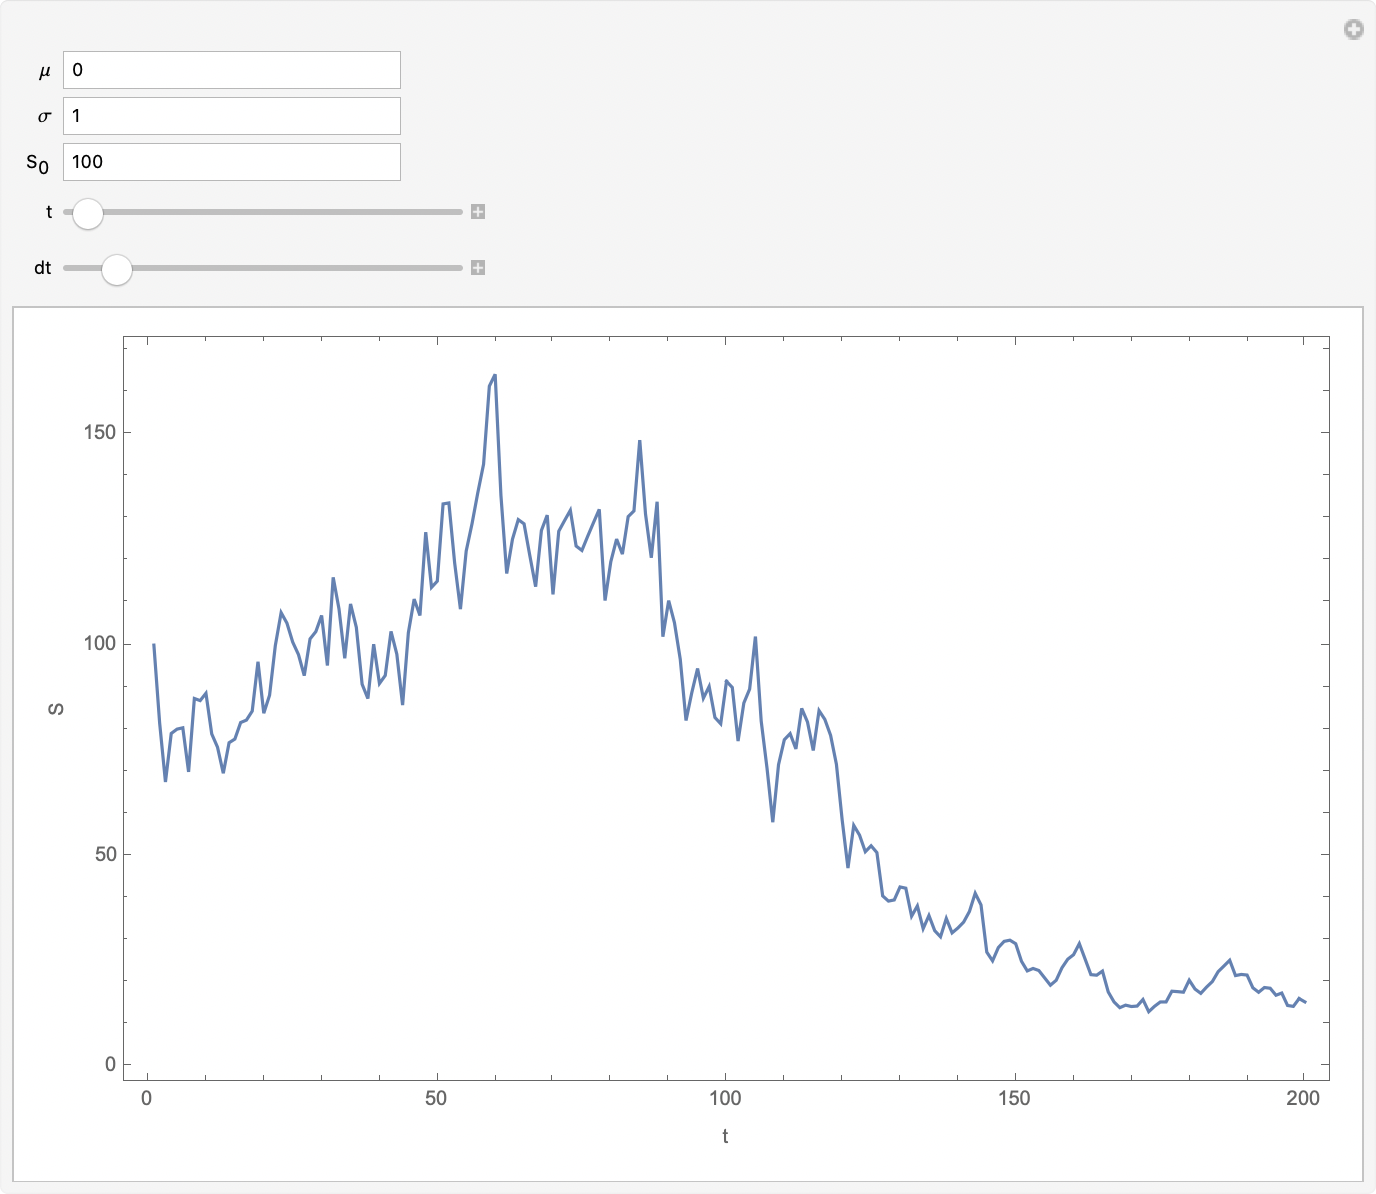
\includegraphics[width=0.7\textwidth]{Wiener.png}
    \caption{Estado inicial de la visualización del proceso de Wiener. Puede verse cómo los distintos parámetros son modificables por el usuario así como la gráfica que se genera.}
    \label{fig:Wiener}
\end{figure}

\item \emph{En un mercado bursátil se acuerda crear una opción llamada “call ventana”, la cual funciona como una opción call europea que se puede ejercer solamente cuando el precio del activo $S$ está en un rango de valores: $E_1 \leq S(T) \leq E_2$ al momento de la madurez (vencimiento) $T$, con un precio strike $E$, incluido en este intervalo. El precio $S$ del activo subyacente se comporta como en el modelo de camino aleatorio dado en el ejercicio 1). Usted debe encontrar la fórmula de valoración $C = C(S,t)$ para valorar una opción ventana con parámetros $T$, $E$, $E_1$ y $E_2$. Para ello siga los siguientes pasos:}

\begin{enumerate}[label=\alph*)]

\item \emph{Plantee la ecuación diferencial parcial de Black-Scholes que rige el precio $C$. Esto hágalo paso a paso y en detalle riguroso, en términos de cálculo estocástico.}

\medskip

\textbf{\textit{Sol.}} Tenemos que el precio $S$ del activo obedecerá la ecuación de un camino aleatorio, $dS = \mu Sdt + \sigma S dX$, mientras que el precio $C$ es una función de $S$ y $t$, luego expandiendo en series de Taylor tenemos

\begin{align*}
    dC = \frac{\partial C}{\partial t}dt + \frac{\partial C}{\partial S} dS + \frac{1}{2}\frac{\partial^2C}{\partial S^2}dS^2,
\end{align*}

y en particular tenemos que $dS$ está dado como antes y para el término $dS^2$ consideramos que $dt^2 \to 0$ y $dtdX \to 0$ pero $dX^2 = \mathcal{O}(dt)$, entonces podemos escribir

\begin{align*}
    dC = \frac{\partial C}{\partial t}dt + \frac{\partial C}{\partial S}(\mu Sdt + \sigma S dX) + \frac{1}{2}\frac{\partial^2C}{\partial S^2}\sigma^2S^2dt,
\end{align*}

y reordenando un poco los términos tenemos finalmente

\begin{align*}
    dC = \left(\frac{\partial C}{\partial t} + \mu S\frac{\partial C}{\partial S} + \frac{\sigma^2S^2}{2}\frac{\partial^2C}{\partial S^2}\right)dt + \sigma S\frac{\partial C}{\partial S}dX,
\end{align*}

esto sencillamente es el lema de Itô.

Ahora queremos eliminar la aleatoriedad, para lo cual consideramos un portafolio $\Pi = C - \Delta S$ sin riesgo, es decir, queremos que su diferencial $d\Pi$ no tenga parte estocástica, vemos entonces la forma de este diferencial

\begin{align*}
    d\Pi &= dC - \Delta dS\\
    &= \left(\frac{\partial C}{\partial t} + \mu S\frac{\partial C}{\partial S} + \frac{\sigma^2S^2}{2}\frac{\partial^2C}{\partial S^2}\right)dt + \sigma S\frac{\partial C}{\partial S}dX - \Delta\left(\mu Sdt + \sigma SdX\right)\\
    &= \left[\frac{\partial C}{\partial t} + \mu S\left(\frac{\partial C}{\partial S} - \Delta\right) + \frac{\sigma^2S^2}{2}\frac{\partial^2C}{\partial S^2}\right]dt + \sigma S\left(\frac{\partial C}{\partial S} - \Delta\right)dX,
\end{align*}

y es claro que para eliminar la parte estocástica sencillamente requerimos $\Delta = \frac{\partial C}{\partial S}$, con lo cual

\begin{align*}
    d\Pi = \left(\frac{\partial C}{\partial t} + \frac{\sigma^2S^2}{2}\frac{\partial^2C}{\partial S^2}\right)dt.
\end{align*}

Por otra parte, dado que por definición $\Pi$ es un portafolio libre de riesgo, también debe ser que $d\Pi = r\Pi dt$ para una tasa libre de riesgo $r$, así

\begin{align*}
    \frac{\partial C}{\partial t} + \frac{\sigma^2S^2}{2}\frac{\partial^2C}{\partial S^2} = rC - rS\frac{\partial C}{\partial S},
\end{align*}

cosa que podemos reordenar en la forma más conocida de la ecuación diferencial parcial de Black-Scholes

\begin{align*}
    \frac{\partial C}{\partial t} + \frac{\sigma^2S^2}{2}\frac{\partial^2C}{\partial S^2} + rS\frac{\partial C}{\partial S} - rC = 0.
\end{align*}

\item \emph{Proponga las condiciones de frontera para $C$.}

\medskip

\textbf{\textit{Sol.}} Para imponer condiciones de frontera consideramos primero el mecanismo mediante el cual se ejerce la opción, i.e., si en el tiempo $T$ se tiene $S(T) < E_1$ o $S(T) > E_2$ no se ejerce e inmediatamente tenemos $C(S,T) = 0$, mientras que si en el tiempo $T$ se tiene $E_1 \leq S(T) \leq E_2$ se ejerce la opción y $C(S,T) = S(T) - E$. Luego consideramos lo que ocurre cuando $S(t) = 0$ y cuando $S(t) \to \infty$, si el valor del subyacente se anula, naturalmente tenemos $C(0,t) = 0$, mientras que si el valor del subyacente sobrepasa el valor de referencia $E_2$, debemos también escribir $C(S_\infty,t) = 0$.

En resumen, tenemos las siguientes condiciones de frontera

\begin{align*}
    C(S,T) &= \begin{cases}
                0, &\qquad S(T) < E_1\\
                S(T) - E, &\qquad E_1 \leq S(T) \leq E_2\\
                0, &\qquad E_2 < S(T)
              \end{cases}\\
    C(0,t) &= 0\\
    C(S_\infty,t) &= 0.
\end{align*}

\item \emph{Transforme la ecuación diferencial parcial de Black-Scholes para $C$ en una ecuación de difusión y resuélvala analíticamente si es posible. Utilice la función de distribución de probabilidad acumulada de una variable aleatoria normal estándar.}

\medskip

\textbf{\textit{Sol.}} Realizamos ahora un cambio de variables según

\begin{align*}
    S &= Ee^x,\\
    t &= T - \frac{\tau}{\sigma^2/2},\\
    C(S,t) &= Ec(x,\tau),
\end{align*}

con lo cual tendremos los diferenciales

\begin{align*}
    \frac{\partial C}{\partial t} &= E\frac{\partial c}{\partial \tau}\frac{\partial \tau}{\partial t}\\
    &= -\frac{E\sigma^2}{2}\frac{\partial c}{\partial\tau},\\
    \frac{\partial C}{\partial S} &= E\frac{\partial c}{\partial x}\frac{\partial x}{\partial S}\\
    &= \frac{E}{S}\frac{\partial c}{\partial x},\\
    \frac{\partial^2 C}{\partial S^2} &= \frac{\partial}{\partial S}\frac{E}{S}\frac{\partial c}{\partial x}\\
    &= -\frac{E}{S^2}\frac{\partial c}{\partial x} + \frac{E}{S}\frac{\partial^2 c}{\partial x^2}\frac{\partial x}{\partial S}\\
    &= -\frac{E}{S^2}\frac{\partial c}{\partial x} + \frac{E}{S^2}\frac{\partial^2 c}{\partial x^2}\\
    &= \frac{E}{S^2}\left(\frac{\partial^2 c}{\partial x^2} - \frac{\partial c}{\partial x}\right),
\end{align*}

y podemos reescribir la ecuación diferencial parcial como

\begin{align*}
    -\frac{\sigma^2}{2}\frac{\partial c}{\partial\tau} + \frac{\sigma^2}{2}\left(\frac{\partial^2 c}{\partial x^2} - \frac{\partial c}{\partial x}\right) + r\frac{\partial c}{\partial x} - rc = 0,
\end{align*}

finalmente definiendo $k = \frac{r}{\sigma^2/2}$ podemos tenerla en la forma

\begin{align*}
    \frac{\partial c}{\partial\tau} = \frac{\partial^2c}{\partial x^2} + (k - 1)\frac{\partial c}{\partial x} - kc.
\end{align*}

Habiendo realizado estas primeras transformaciones, realizamos una nueva transformación según

\begin{align*}
    c(x,\tau) = e^{\alpha x + \beta\tau}u(x,\tau),
\end{align*}

con la cual la ecuación será inicialmente más complicada

\begin{align*}
    \left(\frac{\partial u}{\partial\tau} + \beta u\right) = \left(\frac{\partial^2u}{\partial x^2} + 2\alpha\frac{\partial u}{\partial x} + \alpha^2u\right) + (k - 1)\left(\frac{\partial u}{\partial x} + \alpha u\right) - ku,
\end{align*}

pero puede ordenarse como

\begin{align*}
    \frac{\partial u}{\partial\tau} = \frac{\partial^2u}{\partial x^2} + \left(2\alpha + k - 1\right)\frac{\partial u}{\partial x} + \left(\alpha^2 + \alpha(k - 1) - \beta - k\right)u,
\end{align*}

lo cual permite la estratégica escogencia de los parámetros $\alpha$ y $\beta$ como

\begin{align*}
    \alpha &= \frac{1 - k}{2},\\
    \beta &= -\frac{(k + 1)^2}{4},
\end{align*}

y así la ecuación no será más que

\begin{align*}
    \frac{\partial u}{\partial\tau} = \frac{\partial^2u}{\partial x^2},
\end{align*}

la famosa ecuación del calor en una dimensión.

Por su parte las condiciones de frontera también han de transformarse según se transformó la ecuación, tenemos entonces

\begin{align*}
    c(x,0) &= \begin{cases}
                0, &\qquad x < \log\frac{E_1}{E}\\
                e^x - 1, &\qquad \log\frac{E_1}{E} \leq x \leq \log\frac{E_2}{E}\\
                0, &\qquad \log\frac{E_2}{E} < x
              \end{cases}
\end{align*}

para la primera transformación y luego

\begin{align*}
    u(x,0) &= \begin{cases}
                0, &\qquad x < \log\frac{E_1}{E}\\
                e^{x - \alpha x} - e^{-\alpha x}, &\qquad \log\frac{E_1}{E} \leq x \leq \log\frac{E_2}{E}\\
                0, &\qquad \log\frac{E_2}{E} < x
              \end{cases}
\end{align*}

para la segunda.

Una solución general de la ecuación de calor es la fdp de una variable aleatoria con distribución normal

\begin{align*}
    u(x,\tau) = \frac{1}{2\sqrt{\pi\tau}}e^{-\frac{x^2}{4\tau}},
\end{align*}

y luego para satisfacer las condiciones de frontera buscamos que $u(x,0) = g(x)$ con $g(x)$ definida a trozos como se escribió antes. Notamos que para $\tau \to 0$ la fdp que tenemos se volverá una delta de Dirac por lo que finalmente tendremos la solución

\begin{align*}
    u(x,\tau) = \int_{-\infty}^\infty \frac{1}{2\sqrt{\pi\tau}}e^{-\frac{(x - s)^2}{4\tau}}g(s)ds,
\end{align*}

que no es más que el valor esperado de $g(x)$ respecto a la distribución normal descrita anteriormente.

Por último realizamos la integración aprovechando que $g(x)$ se anula en gran parte de la recta real,

\begin{align*}
    u(x,\tau) &= \int_{\log\frac{E_1}{E}}^{\log\frac{E_2}{E}} \frac{1}{2\sqrt{\pi\tau}}e^{-\frac{(x - s)^2}{4\tau}}(e^{s - \alpha s} - e^{-\alpha s})ds\\
    &= \int_0^{\log\frac{E_2}{E}} \frac{1}{2\sqrt{\pi\tau}}e^{-\frac{(x - s)^2}{4\tau}}(e^{s - \alpha s} - e^{-\alpha s})ds\\
    &\quad - \int_0^{\log\frac{E_1}{E}} \frac{1}{2\sqrt{\pi\tau}}e^{-\frac{(x - s)^2}{4\tau}}(e^{s - \alpha s} - e^{-\alpha s})ds,
\end{align*}

y simplificando mediante la transformación $s = x + \sqrt{2\tau}y$ tenemos

\begin{align*}
    u(x,\tau) &= \int_{-\frac{x}{\sqrt{2\tau}}}^{\frac{1}{\sqrt{2\tau}}\left(\log\frac{E_2}{E} - x\right)} \frac{1}{\sqrt{2\pi}}e^{-\frac{y^2}{2}}(e^{x + \sqrt{2\tau}y - \alpha(x + \sqrt{2\tau}y)} - e^{-\alpha(x + \sqrt{2\tau}y)})dy\\
    &\quad - \int_{-\frac{x}{\sqrt{2\tau}}}^{\frac{1}{\sqrt{2\tau}}\left(\log\frac{E_1}{E} - x\right)} \frac{1}{\sqrt{2\pi}}e^{-\frac{y^2}{2}}(e^{x + \sqrt{2\tau}y - \alpha(x + \sqrt{2\tau}y)} - e^{-\alpha(x + \sqrt{2\tau}y)})dy\\
    &= \int_{-\frac{x}{\sqrt{2\tau}}}^{\frac{1}{\sqrt{2\tau}}\left(\log\frac{E_2}{E} - x\right)} \frac{1}{\sqrt{2\pi}}e^{-\frac{y^2}{2}}e^{x + \sqrt{2\tau}y - \alpha(x + \sqrt{2\tau}y)}dy\\
    &\quad - \int_{-\frac{x}{\sqrt{2\tau}}}^{\frac{1}{\sqrt{2\tau}}\left(\log\frac{E_2}{E} - x\right)} \frac{1}{\sqrt{2\pi}}e^{-\frac{y^2}{2}}e^{-\alpha(x + \sqrt{2\tau}y)}dy\\
    &\qquad - \int_{-\frac{x}{\sqrt{2\tau}}}^{\frac{1}{\sqrt{2\tau}}\left(\log\frac{E_1}{E} - x\right)} \frac{1}{\sqrt{2\pi}}e^{-\frac{y^2}{2}}e^{x + \sqrt{2\tau}y - \alpha(x + \sqrt{2\tau}y)}dy\\
    &\qquad + \int_{-\frac{x}{\sqrt{2\tau}}}^{\frac{1}{\sqrt{2\tau}}\left(\log\frac{E_1}{E} - x\right)} \frac{1}{\sqrt{2\pi}}e^{-\frac{y^2}{2}}e^{-\alpha(x + \sqrt{2\tau}y)}dy\\
    &= \frac{e^{x - \alpha x}}{\sqrt{2\pi}} \int_{-\frac{x}{\sqrt{2\tau}}}^{\frac{1}{\sqrt{2\tau}}\left(\log\frac{E_2}{E} - x\right)} e^{-\frac{y^2}{2}}e^{\sqrt{2\tau}y - \alpha\sqrt{2\tau}y}dy\\
    &\quad - \frac{e^{-\alpha x}}{\sqrt{2\pi}}\int_{-\frac{x}{\sqrt{2\tau}}}^{\frac{1}{\sqrt{2\tau}}\left(\log\frac{E_2}{E} - x\right)} e^{-\frac{y^2}{2}}e^{-\alpha\sqrt{2\tau}y}dy\\
    &\qquad - \frac{e^{x - \alpha x}}{\sqrt{2\pi}} \int_{-\frac{x}{\sqrt{2\tau}}}^{\frac{1}{\sqrt{2\tau}}\left(\log\frac{E_1}{E} - x\right)} e^{-\frac{y^2}{2}}e^{\sqrt{2\tau}y - \alpha\sqrt{2\tau}y}dy\\
    &\qquad + \frac{e^{-\alpha x}}{\sqrt{2\pi}} \int_{-\frac{x}{\sqrt{2\tau}}}^{\frac{1}{\sqrt{2\tau}}\left(\log\frac{E_1}{E} - x\right)} e^{-\frac{y^2}{2}}e^{-\alpha\sqrt{2\tau}y}dy,
\end{align*}

una última transformación análoga a la anterior nos da

\begin{align*}
    u(x,\tau) &= \frac{e^{-(\alpha - 1)x + (\alpha - 1)^2\tau}}{\sqrt{2\pi}} \int_{(\alpha - 1)\sqrt{2\tau} - \frac{x}{\sqrt{2\tau}}}^{\frac{1}{\sqrt{2\tau}}\left(\log\frac{E_2}{E} - x\right) + (\alpha - 1)\sqrt{2\tau}} e^{-\frac{w^2}{2}}dw\\
    &\quad - \frac{e^{-\alpha x + \alpha^2\tau}}{\sqrt{2\pi}}\int_{\alpha\sqrt{2\tau} - \frac{x}{\sqrt{2\tau}}}^{\frac{1}{\sqrt{2\tau}}\left(\log\frac{E_2}{E} - x\right) + \alpha\sqrt{2\tau}} e^{-\frac{w^2}{2}}dw\\
    &\qquad - \frac{e^{-(\alpha - 1)x + (\alpha - 1)^2\tau}}{\sqrt{2\pi}} \int_{(\alpha - 1)\sqrt{2\tau} - \frac{x}{\sqrt{2\tau}}}^{\frac{1}{\sqrt{2\tau}}\left(\log\frac{E_1}{E} - x\right) + (\alpha - 1)\sqrt{2\tau}} e^{-\frac{w^2}{2}}dw\\
    &\qquad + \frac{e^{-\alpha x + \alpha^2\tau}}{\sqrt{2\pi}} \int_{\alpha\sqrt{2\tau} - \frac{x}{\sqrt{2\tau}}}^{\frac{1}{\sqrt{2\tau}}\left(\log\frac{E_1}{E} - x\right) + \alpha\sqrt{2\tau}} e^{-\frac{w^2}{2}}dw,
\end{align*}

lo cual nos permite escribir todo en términos de la fdc $F$ de una normal estándar como

\begin{align*}
    u(x,\tau) &= e^{-(\alpha - 1)x + (\alpha - 1)^2\tau}\left[F\left(\frac{\log\frac{E_2}{E} - x}{\sqrt{2\tau}} + (\alpha - 1)\sqrt{2\tau}\right) - F\left(\frac{\log\frac{E_1}{E} - x}{\sqrt{2\tau}} + (\alpha - 1)\sqrt{2\tau}\right)\right]\\
    &\quad - e^{-\alpha x + \alpha^2\tau}\left[F\left(\frac{\log\frac{E_2}{E} - x}{\sqrt{2\tau}} + \alpha\sqrt{2\tau}\right) - F\left(\frac{\log\frac{E_1}{E} - x}{\sqrt{2\tau}} + \alpha\sqrt{2\tau}\right)\right].
\end{align*}

Por último reversamos todas las transformaciones que se aplicaron a la ecuación diferencial parcial original para llegar a una solución de ésta

\begin{align*}
    C(S,t) &= S\left[F\left(\frac{\log\frac{E_2}{S} - \left(r + \frac{\sigma^2}{2}\right)(T - t)}{\sigma\sqrt{T - t}}\right) - F\left(\frac{\log\frac{E_1}{S} - \left(r + \frac{\sigma^2}{2}\right)(T - t)}{\sigma\sqrt{T - t}}\right)\right]\\
    &\quad - Ee^{-r(T - t)}\left[F\left(\frac{\log\frac{E_2}{S} - \left(r - \frac{\sigma^2}{2}\right)(T - t)}{\sigma\sqrt{T - t}}\right) - F\left(\frac{\log\frac{E_1}{S} - \left(r - \frac{\sigma^2}{2}\right)(T - t)}{\sigma\sqrt{T - t}}\right)\right].
\end{align*}

\item \emph{Dibuje claramente la superficie de la función $C = C(S,t)$ para diferentes valores de la tasa libre de riesgo y la volatilidad (sigma).}

\medskip

\textbf{\textit{Sol.}} Se dibujó la superficie correspondiente a la función $C = C(S,t)$ para algunos valores distintos de $\sigma$ y de $r$, las gráficas resultantes pueden verse en la figura \ref{fig:Surf}.

\begin{figure}[h!]
\centering
\begin{minipage}{0.49\textwidth}
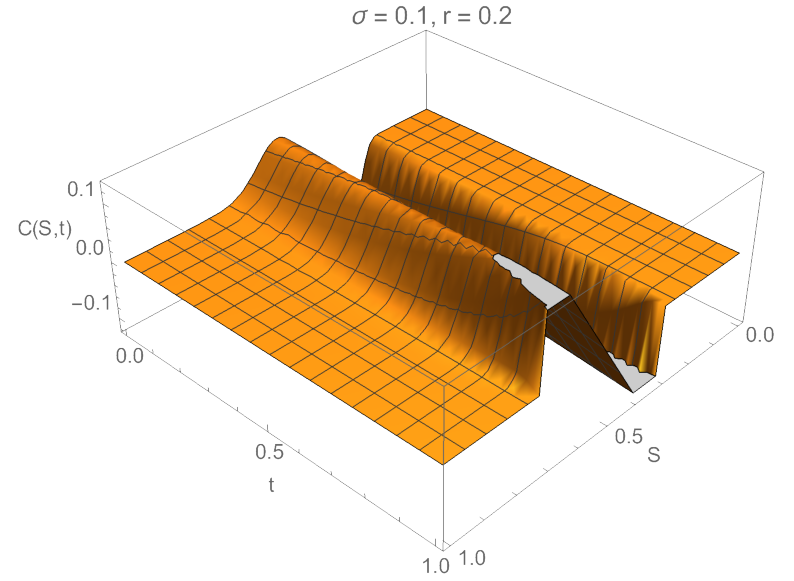
\includegraphics[width=0.8\textwidth]{surf1.pdf}
\end{minipage}
\begin{minipage}{0.49\textwidth}
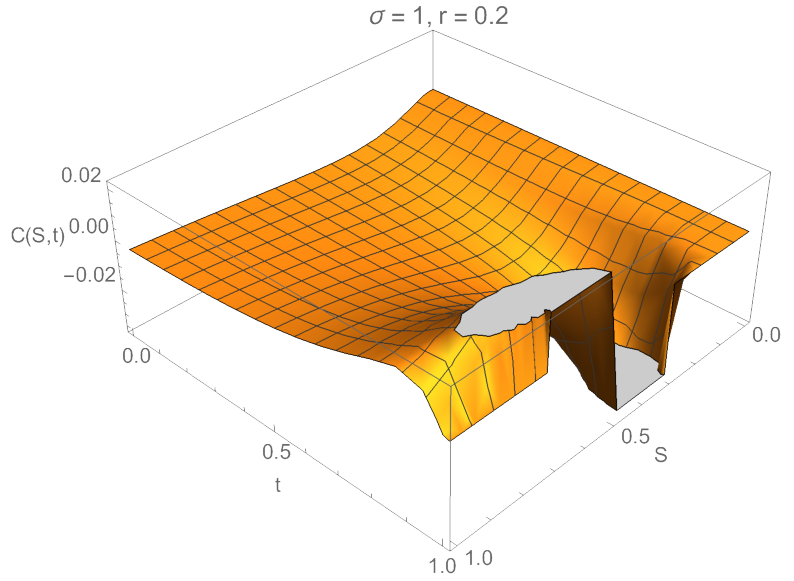
\includegraphics[width=0.8\textwidth]{surf2.pdf}
\end{minipage}
\begin{minipage}{0.49\textwidth}
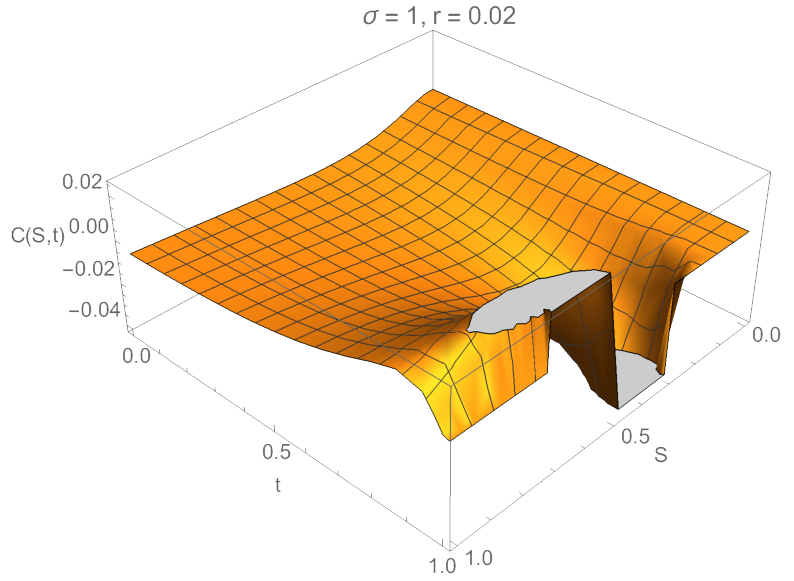
\includegraphics[width=0.8\textwidth]{surf3.pdf}
\end{minipage}
\begin{minipage}{0.49\textwidth}
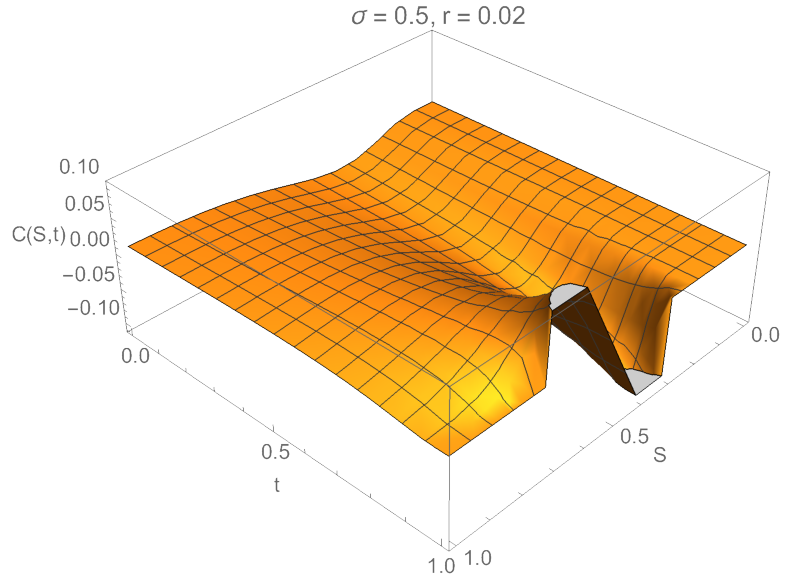
\includegraphics[width=0.8\textwidth]{surf4.pdf}
\end{minipage}
\caption{Superficies de la función $C = C(S,t)$.}
\label{fig:Surf}
\end{figure}

\end{enumerate}

\item \emph{Utilizando la función de valoración $C = C(S,t)$ para opciones ventana sobre el
subyacente $S$ que usted calculó, componga un portafolio que incluya activos sin riesgo (a la tasa libre de riesgo), inversiones en el activo $S$ e inversiones en la opción ventana sobre el subyacente representado por $S$. Para la composición de su portafolio, simule la evolución del valor de éste, empleando el módulo de simulación para $S$ del problema 1) y la fórmula de valoración de la opción ventana. Considere diferentes valores para los parámetros de tasa libre de riesgo y volatilidad. Demuestre que esto hace el portafolio más seguro en general con varias simulaciones.}

\medskip

\textbf{\textit{Sol.}} 

\item \emph{Enuncie y demuestre rigurosamente la fórmula de paridad call-put acorde a las lecturas.}

\medskip

\textbf{\textit{Sol.}} 

\end{enumerate}

\end{document}